\documentclass[12pt]{article}
\usepackage[utf8]{inputenc}
\usepackage{amsmath}
\usepackage{algorithm}
\usepackage{graphicx}
\graphicspath{ {images/} }
\usepackage{hyperref}
\usepackage{amsmath}

\usepackage{algorithm}
\usepackage{algorithmicx}
\usepackage{algpseudocode}

\usepackage{listings}
\usepackage{xcolor}
\usepackage{textcomp}
\usepackage{amssymb}
\usepackage{url}

\usepackage[framed,numbered,autolinebreaks,useliterate]{mcode}


\title{ENGN4528/6528 Computer Vision – 2015 Computer-Lab 5 (C-Lab5)}
\author{Sai Ma - u5224340}
\date{May 2015}

\floatname{algorithm}{Algorithm}
\renewcommand{\algorithmicrequire}{\textbf{input:}}
\renewcommand{\algorithmicensure}{\textbf{output:}}

\begin{document}

\maketitle


\section{Camera Calibration}
In this task, we asked to develop a method to calibrate camera, finding the relationship between 3D world coordiantes and their 2D projection positions in the image. In this task, we needs two sets of points. We select the 2D coordinate points on a testing image (e.g. \textit{stereo2012a.jpg}) by Matlab method \textit{ginput()}. At the same time, we construct a 3D coordiante points information based on given image displayed information. The calibration target image has three mutually orthogonal faces with marked points. These points are located on the regular grid, and apart from $7$ cm. Therefore, we construct \textit{original} point coordinates in these grids. We can build the 3D system as figure \ref{fig:stereo2012aWithPoints} shown.

\begin{figure}[h]
    \centering
    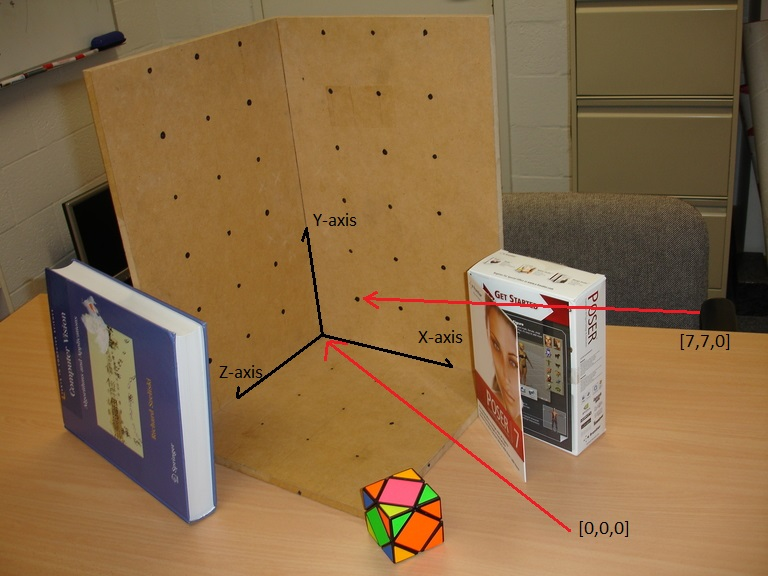
\includegraphics[width=0.8\textwidth]{stereo2012aWithPoints.jpg}
    \caption{Stereo2012a With 3D Coordinate System}
    \label{fig:stereo2012aWithPoints}
\end{figure}

Therefore, I create $12$ 3D points in this coordinate system, and select their corresponding image location to get their 2D points coordinates. In order to use them easily, I also use Matlab method \textit{load} and \textit{save} to save and load these arguments.


\begin{lstlisting}
% for the XYZ, it is constructed by ourselve, we use same XYZ system in two
% different images
XYZ = [0,7,7; 0,7,14; 0,14,14; 0,14,7; 0,21,7; 0,21,14;
       7,7,0; 14,7,0; 14,14,0; 7,14,0; 7,21,0; 14,21,0];
       
% read image, and build uv system
imageName1 = 'stereo2012a.jpg';
img = imread(imageName1);

figure('name', imageName1);
imshow(img);
hold on

% select 12 points from this image
[u1, v1] = ginput(12);

change uv to input style
uv = [u1, v1];
save('stereo2012a.mat', 'uv');

load('stereo2012a.mat');
\end{lstlisting}

Then, the next job is to construct method named \textit{calibrate()}. Its inputs are 3D coordinate points, 2D coordinate points and image. As the lecture taught, we use 3D points $XYZ$ and 2D points $uv$ to construct these $n$ $2\times 12$ matrices $A_{i}$, then merge into a single $2n \times 12$ matrix $A$. Then we compute SVD of $A$, then get our solution $P$ at last column of $V$. 

\begin{lstlisting}
%In this method, the main task is constract matrix A, then get p 
[pointNum, ~] = size(uv);
    
A = zeros(pointNum*2, 12);

for AIndex = 1 : pointNum
    
    X = XYZ(AIndex, 1);
    Y = XYZ(AIndex, 2);
    Z = XYZ(AIndex, 3);
        
    u = uv(AIndex, 1);
    v = uv(AIndex, 2);
        
    A(AIndex*2 - 1, :) = [X, Y, Z, 1, 0, 0, 0, 0, -u*X, -u*Y, -u*Z, -u];
    A(AIndex*2, :) = [0, 0, 0, 0, X, Y, Z, 1, -v*X, -v*Y, -v*Z, -v];
        
end
    
[~, ~, V] = svd(A,0);    
P = reshape(V(:,end), 4, 3)';
\end{lstlisting}

Then, we get our target $P$. In order to prove that we get the correct $P$, I plan to multiply 3D points by $P$, and get transformed $uv$ points. At the same time, we can calculate mean square error between $uv$ and $uvTrans$. Then, we plot original and transformed points on the image to compare distances between these points.

\begin{lstlisting}
% then, write a method to get reprojection error, get our transformed
% points
XYZone = [XYZ, ones(pointNum, 1)]'; % construct XYZone with four columns
uvTrans = P*XYZone; % get transformed uv values
uvTrans(1,:) = uvTrans(1,:)./uvTrans(3,:); % make transformed uv third row is 1
uvTrans(2,:) = uvTrans(2,:)./uvTrans(3,:);

% get Euclidean distance between re-projected points and original points
reprojectError = sqrt(sum(sum((uvTrans(1:2,:) - uv').^2)));
    
fprintf('The mean reprojection error is: %d.\n', reprojectError/pointNum);
    
% also show our select points in image, with coordinate calcuated by P
uvTrans = uvTrans';
    
figure('Name', 'Selection Points Compare with Calcuated Points');
imshow(im);
hold on;
plot(uv(:,1),uv(:,2),'g+');
plot(uvTrans(:,1),uvTrans(:,2),'ro');
hold off;
\end{lstlisting}

The following figure \ref{fig:stereo2012aResult} and figure \ref{fig:stereo2012bResult} are these compared results.

\begin{figure}[h]
    \centering
    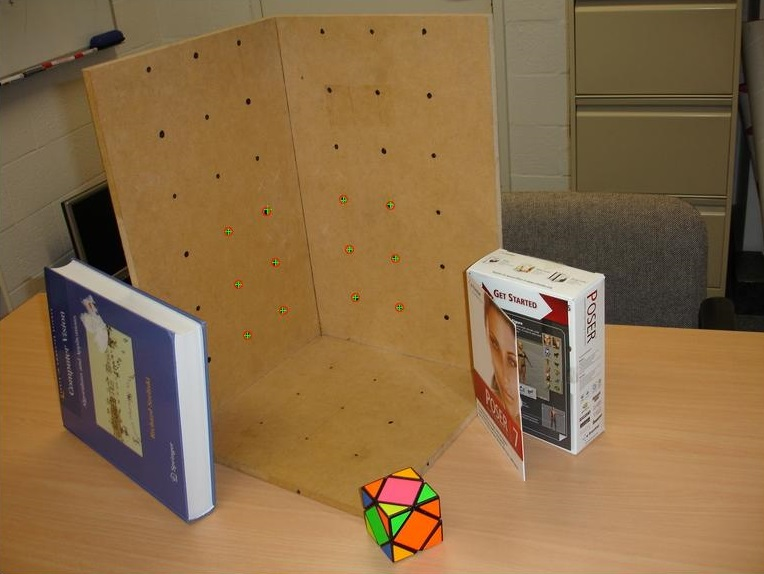
\includegraphics[width=0.9\textwidth]{stereo2012aResult.jpg}
    \caption{Stereo2012a Original Points and Transformed Points}
    \label{fig:stereo2012aResult}
\end{figure}

\begin{figure}[h]
    \centering
    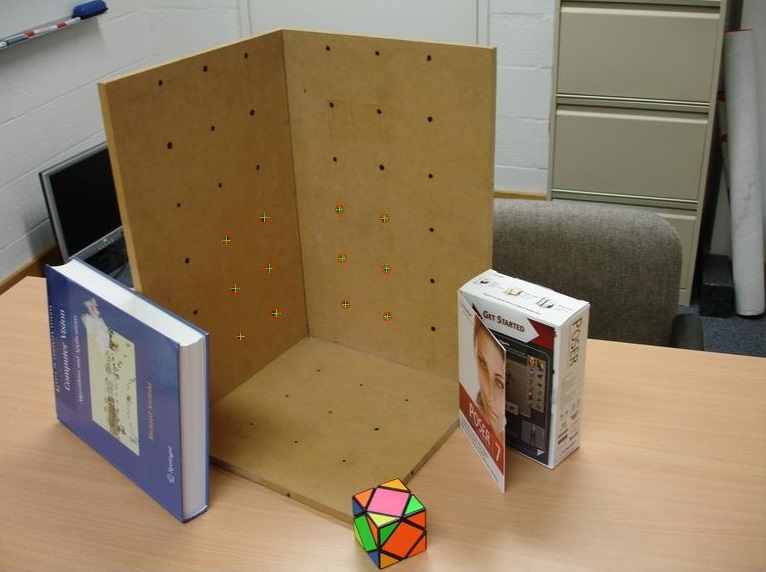
\includegraphics[width=0.9\textwidth]{stereo2012bResult.jpg}
    \caption{Stereo2012b Original Points and Transformed Points}
    \label{fig:stereo2012bResult}
\end{figure}

\subsection{Q1: List the Basic Derivation of DLT algorithm}

In the DLT algorithm, we have 2D and 3D point pairs, and we aim to get $P$ where $x_{i}$ = $PX_{i}$. In the equation, the $x_{i}$ mean the $i$ 2D coordinates, and the $X_{i}$ mean $i$ 3D coordinate come from point pairs. The $x$ is 2D point, and we change it to $(x,y,w)^{T}$. Consider we can get $x_{i} \times PX_{i}$ = $0$ from original equation. Then we construct the relationship \ref{eq:eq1} that:

\begin{center}
\label{eq:eq1}
$x_{i} \times PX_{i} = \begin{bmatrix} y_{i}p_{3}^{T}X_{i} - w_{i}p_{2}^{T}X_{i} \\ w_{i}p_{1}^{T}X_{i} - x_{i}p_{3}^{T}X_{i} \\ x_{i}p_{2}^{T}X_{i} - y_{i}p_{1}^{T}X_{i} \end{bmatrix}$
\end{center}

where $[p_{i}, p_{2}, p_{3}]^{T}$ equals to $P_{i}$.

When we perform factorize unknowns arguments, we get the equation \ref{eq:eq2} is:

\begin{center}
\label{eq:eq2}
$\begin{bmatrix} 0^{T} & - w_{i}X_{i}^{T} & y_{i}X_{i}^{T} \\ w_{i}X_{i}^{T} & 0^{T} & - x_{i}X_{i}^{T} \\ -y_{i}X_{i}^{T} & x_{i}X_{x}^{T} & 0^{T} \end{bmatrix} \begin{bmatrix}
p_{1} \\ p_{2} \\ p_{3} \end{bmatrix} = A_{i}p = 0$
\end{center}

In this problem, we only need first two line of equations to solve the $p$. Then we aims to solve the equation \ref{eq:eq3}
\begin{center}
\label{eq:eq3}
$\begin{bmatrix} 0^{T} & - w_{i}X_{i}^{T} & y_{i}X_{i}^{T} \\ w_{i}X_{i}^{T} & 0^{T} & - x_{i}X_{i}^{T}\end{bmatrix} \begin{bmatrix}
p_{1} \\ p_{2} \\ p_{3} \end{bmatrix} = A_{i}p = 0$
\end{center}

This matrix $A$ has $11$ degree of freedom, and we need $6$ pairs of 2D and 3D points to solve this $p$, and its solution is 1D nullspace from singular value decomposition of matrix $A$.

\subsection{Q2: Minimally Points and Mean Squared Error}

In our target $P$, it is a $3 \times 4$ matrix and defines as:

\begin{center}
$\begin{bmatrix} p_{00} & p_{01} & p_{02} & p_{03} \\  p_{10} & p_{11} & p_{12} & p_{13} \\  p_{20} & p_{21} & p_{22} & p_{23} \end{bmatrix}$
\end{center}

And once we divide $p$ by $p_{23}$, and this matrix has $11$ unknown arguments. As we known, the $11$ degree of freedom matrix require $11$ point coordinates to solve, and which means $6$ pairs of 2D and 3D point coordinates. As a result, in order to solve this $P$ in 3D DLT, we require at least $6$ pairs of 2D and 3D points.

In the image $stereo2012a.jpg$, my solution on $p$ is:

\begin{center}
$\begin{bmatrix} 0.008253 & -0.004482 & -0.013989 & 0.694305 \\ -0.000617e-4 & -0.015833 & 0.001591 & 0.719304 \\  -1.136248e-05 & -8.123602e-06 & -1.610913e-05 & 0.002155 \end{bmatrix}$
\end{center}

with the mean square error is: $0.189501$.

In the image $stereo2012b.jpg$, my solution on $p$ is:

\begin{center}
$\begin{bmatrix} 0.008564 & -0.004041 & -0.012489 & 0.677494 \\ 0.000483 & -0.015776 & 0.002773 & 0.735183 \\  -9.514198e-06 & -9.034940e-06 &-1.116055e-05 & 0.002171 \end{bmatrix}$
\end{center}

with the mean square error is: $0.268517$.

\subsection{Q3: Decompose P to K, R, t}
\label{sec:decompose}

In the process of decomposition of camera matrix $P$ to $K$, $R$ and $t$ , we have the relationship on camera projection matrix is:

\begin{center}
$P = KR[I | - \tilde{C}]$
\end{center}

where $C$ is the camera center and expressed as $C = (\tilde{C}, 1)$, $K$ is the calibration matrix. Then, the calibration matrix can be obtained from a \textit{RQ decomposition} of the first $3 \times 3$ sub matrix of the camera matrix P. The reason is that $K$ states as:

\begin{center}

$K = \begin{bmatrix} \alpha_{x} & s & x_{0} \\  ~ & \beta_{x} & y_{0} \\  ~ & ~ & 1 \end{bmatrix}$

\end{center}

The $K$ is an upper triangular. At the same time, $R$ is the orthogonal rotation matrix between the camera and world coordinate frames. On the other hand, we have a $3 \times 4$camera projection matrix $P$, then:

\begin{center}
$P = [M | -M\tilde{C}] = M[I | -\tilde{C}]]$
\end{center}

Where $M$ is the first $3 \times 3$ sub matrix of $P$. Compare with first camera projection matrix, we can achieve calibration matrix $K$ and $R$ via RQ decomposition of the first $3 \times 3$ sub matrix of the camera matrix $P$. This can write in Matlab as:

\begin{lstlisting}
N = size(P,1);
M = P(:,1:N);

[K,R] = vgg_rq(M);
\end{lstlisting}

Where the method named \textit{vgg\_rg(H)} perform RQ decomposition of $M$.

\begin{lstlisting}
function [ K, R ] = vgg_rq( M )
% This method used to calcuated the K and R value based on given homography
% matrix.

    M = M';
    [R, K] = qr(M(end:-1:1,end:-1:1)); % perform Orthogonal-triangular decomposition.
    
    R = R';

    R = R(end:-1:1,end:-1:1);
    K = K';
    
    K = K(end:-1:1,end:-1:1);
    
    if det(R)<0
        K(:,1) = -K(:,1);
        R(1,:) = -R(1,:);
    end
end
\end{lstlisting}

At the same time, $P = K*R[eye(3), -t]$. And $K*R$ is the first $3 \times 3$ sub-matrix. Then, we have new equation that $P[:, 4] = M*-t$. Therefore, we write Matlab code as:

\begin{lstlisting}
t = -P(:,1:N)\P(:,end);
\end{lstlisting}

Moreover, we need to recover the camera's focal length. we can check image property in operation system, and its get physical focal length. This camera focal length is $8$ mm.

In the figure \textit{stereo2012a,jpg}, its $K$ (keep its right-down value is $1$)is:

\begin{center}
$\begin{bmatrix} 	
	698.4756172   & 9.234292    & 369.510906 \\  
	     0     & 706.620628   & 241.9471017 \\  
		 0     & 	 0 	    & 1     
\end{bmatrix}$
\end{center}

The $R$ is:

\begin{center}
$\begin{bmatrix} 	
	0.834251 & -0.087245 & -0.544437 \\  
	0.141517 & -0.920446 &  0.364349 \\  
   -0.532913 & -0.381006 & -0.755537
\end{bmatrix}$
\end{center}

Then, our next task is to extract rotated angle from $R$ based on the relationship that:

\begin{center}
$R_{x}(\alpha) = \begin{bmatrix} 1 & 0 & 0 \\  0 & cos\alpha & -sin\alpha \\  0 & sin\alpha & cos\alpha \end{bmatrix}$
\end{center}

\begin{center}
$R_{y}(\beta) = \begin{bmatrix} cos\beta & 0 & sin\beta \\  0 & 1 & 0 \\  -sin\beta & 0 & cos\beta \end{bmatrix}$
\end{center}

\begin{center}
$R_{z}(\gamma) = \begin{bmatrix} cos\gamma & -sin\gamma & 0 \\  sin\gamma & cos\gamma & 0 \\  0 & 0 & 1 \end{bmatrix}$
\end{center}

Then, we extract $\alpha$, $\beta$ and $\gamma$ from $R$ \footnote{use a Matlab method download from \url{http://in.mathworks.com/matlabcentral/fileexchange/43907-compose---decompose-3x3-rotation-matrix--comp-decomp-matrix-}}. The $\alpha$ is: $-153.23$ degrees, $\beta$ is $32.20$ degrees and $\gamma$ is $9.62$ degrees. And the $t$ is $[57.86; 49.99; 67.75]$.

\subsection{Q4: List Second Camera Relative Orientation and Translation}

In the picture \textit{stere2012b.jpg}, we can extract its $t$, $R$ as section \ref{sec:decompose} (the two image have same $K$ as we assumed in question). Then, the $R$ is:

\begin{center}
$\begin{bmatrix} 	
	0.790391 & -0.082483 & -0.607023 \\  
	0.264951 & -0.847394 &  0.460134 \\  
   -0.552341 & -0.524518 & -0.647919
\end{bmatrix}$
\end{center}

Then, we also perform Matlab method \textit{comp\_decomp\_matrix()} to extract $\alpha$ is $-141.00$ degrees, $\beta$ is $33.52$ degrees and $\gamma$ is $18.53$ degrees. And the camera located $t$ is $[-0.64; 63.29; 82.59]$. As a result, we can notice when relative to first camera, the second camera rotate angles are change from $-153.23$ to $-141.00$ at $\alpha$, $32.20$ to $33.5$ at $\beta$ and $9.62$ to $18.53$. And camera translated location are change from $[57.86; 49.99; 67.75]$ to $[-0.64; 63.29; 82.59]$.

\subsection{Q5: Fundamental Matrix}

Fundamental matrix is a $3 \times 3$ matrix of rank $2$. Therefore, its size is $3 \times 3$. Its degree of freedom is $7$. We need $7$ pairs of points coordinates to estimate this fundamental matrix.

\section{Appendix: Matlab Code} 
\label{App:AppendixA}

\lstinputlisting{task1.m}
\lstinputlisting{calibrate.m}
\lstinputlisting{vgg_KR_from_P.m}
\lstinputlisting{comp_decomp_matrix.m}

\end{document}